% ||||||||||||||||||||||||||||||||||||||||||||||
% Capitulo de análise dos resultados
% ||||||||||||||||||||||||||||||||||||||||||||||
\chapter{Análise dos Resultados}

Nesse capítulo apresenta-se os principais resultados e as análises sobre eles, onde serão demostrados os resultados pelos métodos clássicos de sintonia, o desenvolvido nesse trabalho e por fim, uma comparação entre todos.

%%%%%%%%%%%%%%%%%%%%%%%%%%%%%%%%%%%

\subsection{Métodos Clássicos de Sintonia}

Dentre eles, se encontram os métodos de sintonia de Ziegler-Nichols em malha fechada e o Método do Relé. O método de sintonia em malha aberta não pode ser aplicado nesse trabalho, pois em malha aberta, o sistema é instável, ou seja, ao colocarmos uma determinada largura de pulso e não modularmos ela, o simulador de satélite simplesmente ficará girando descontroladamente, pois não existem forças no eixo z para pararem o satélite, como acontece quando um objeto é acelerado no espaço na ausência de forças. Na figura \ref{fig:relay} (a), podemos ver o resultado da aplicação do método do relé em um degrau de amplitude de $\SI{45}{\degree}$, valor esse, usado em todos os ensaios.

\begin{figure}[H]
  \caption{Resultados do método do relé.}
  \begin{center}
      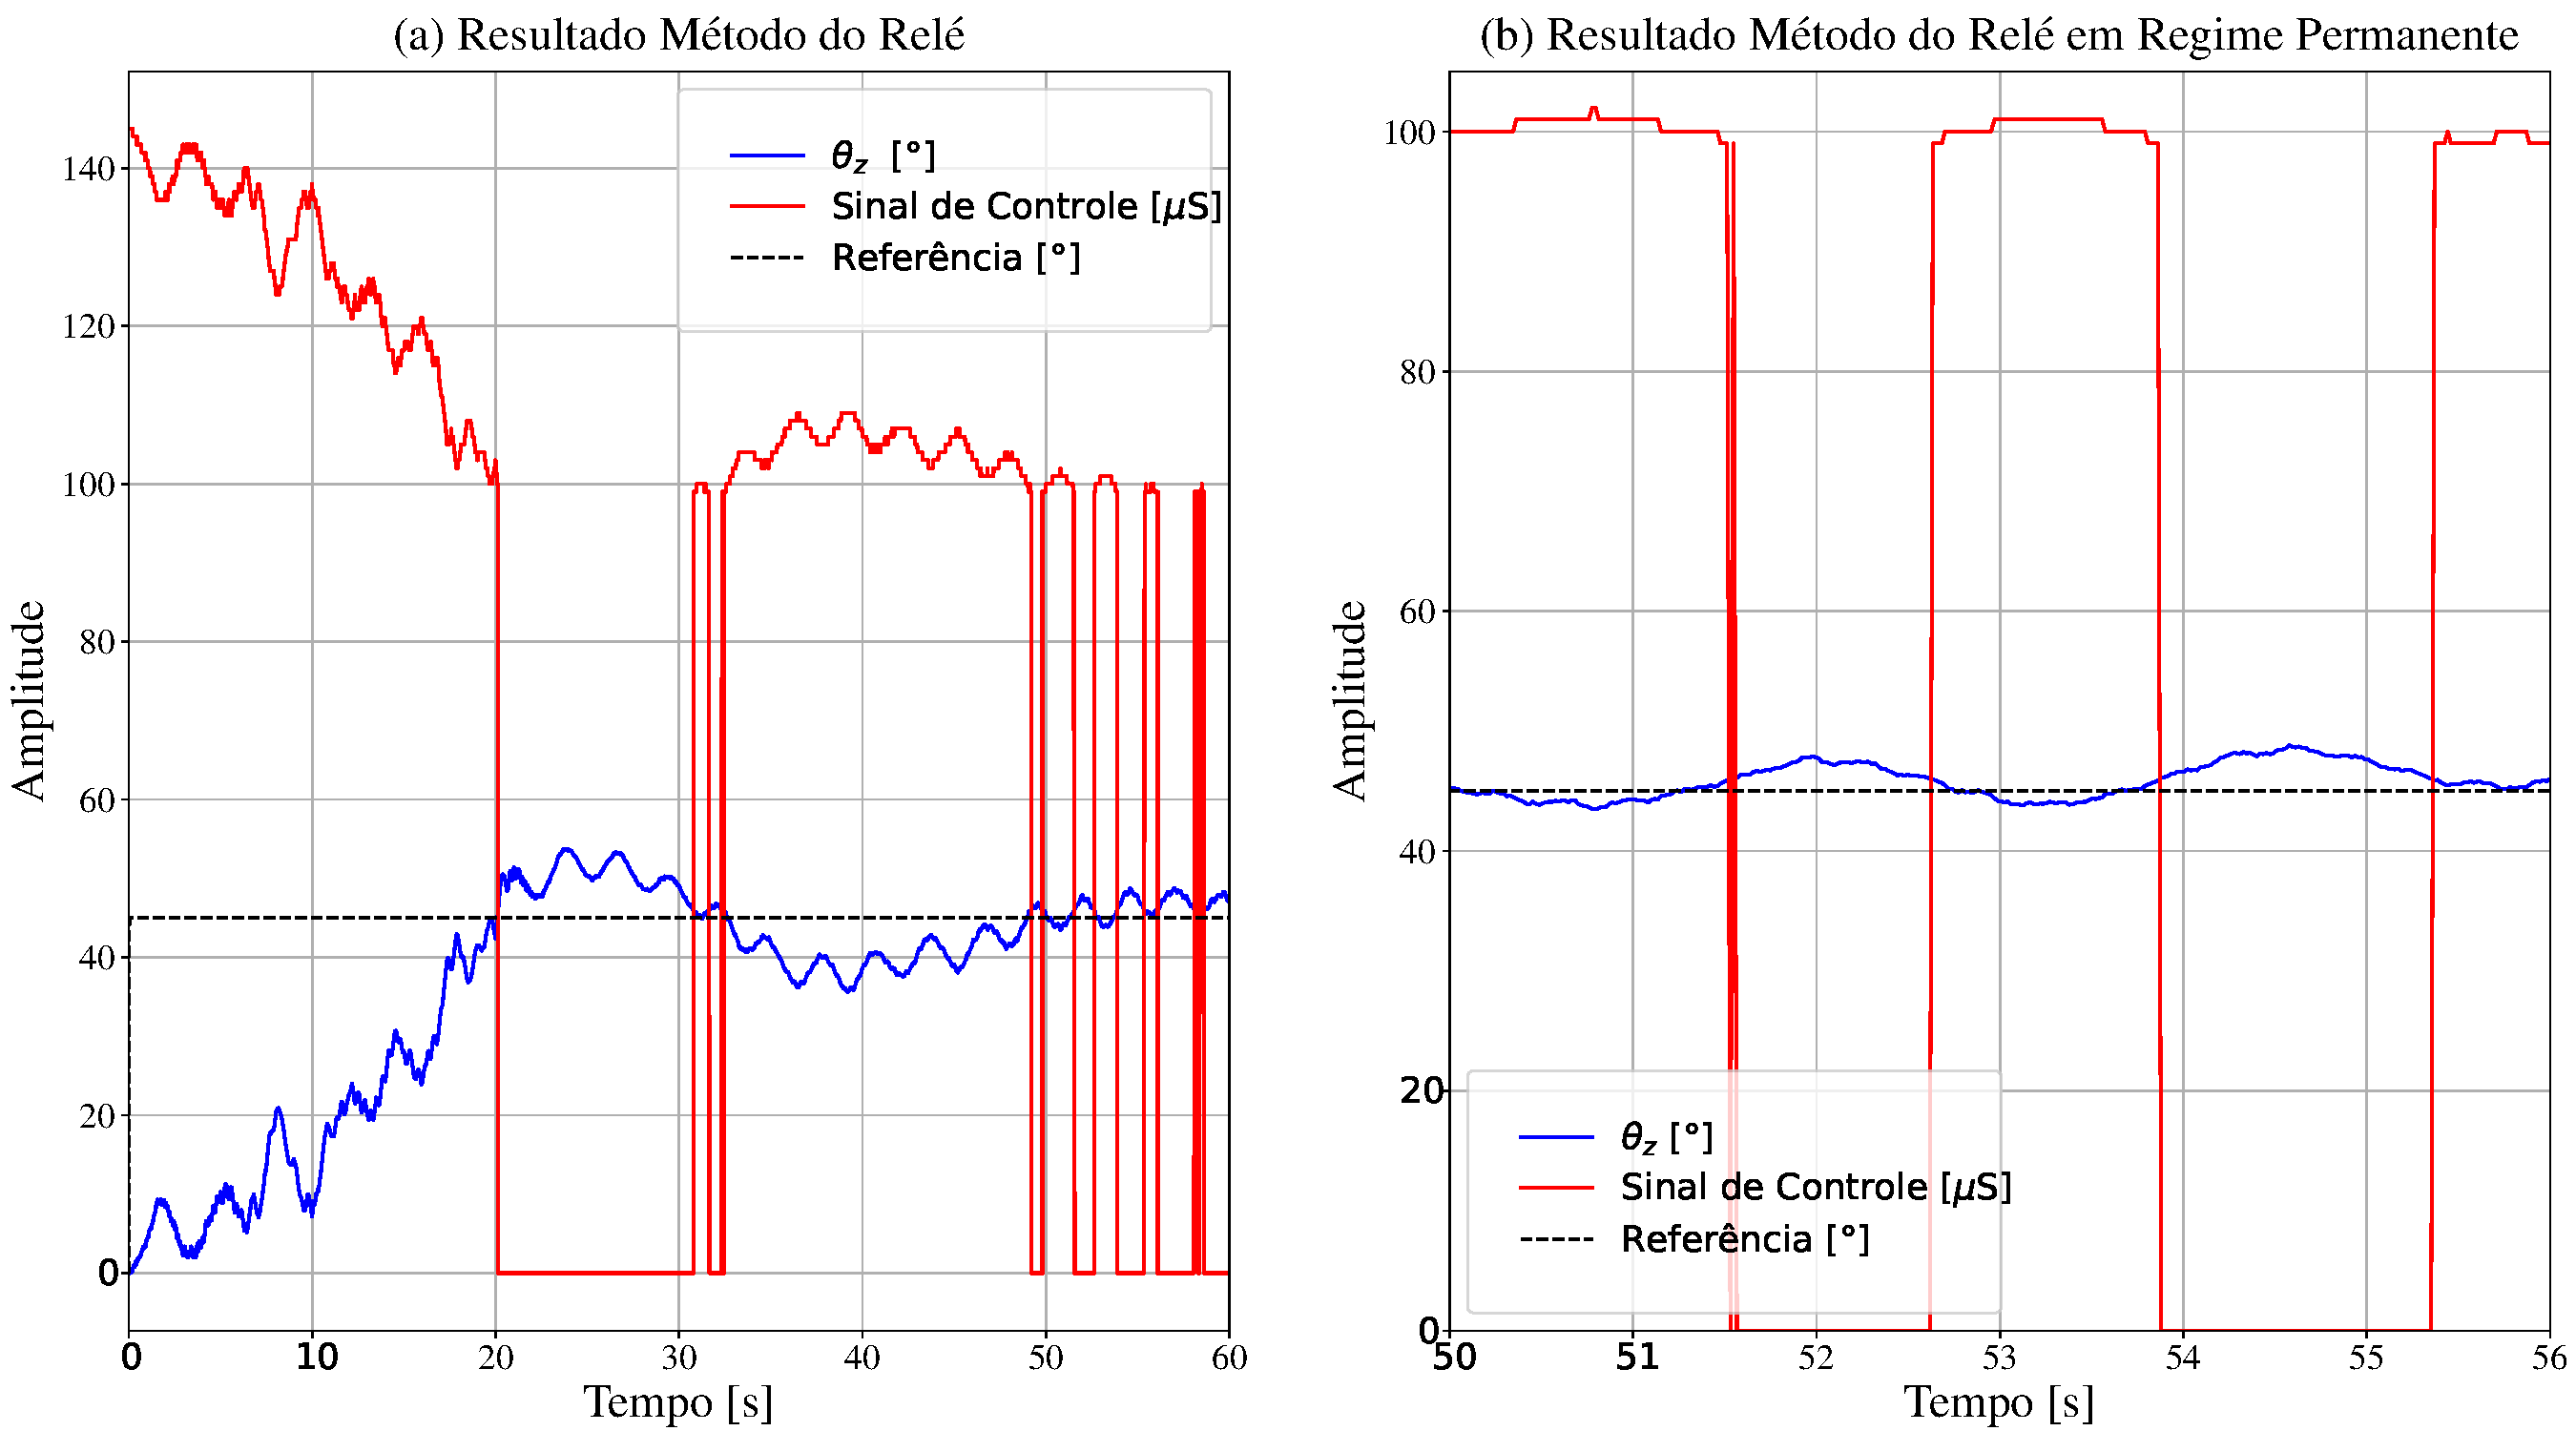
\includegraphics[scale=0.35]{resultados/img/relay}
  \end{center}
  \fonte{Elaborado pelo Autor.} 
  \label{fig:relay}
\end{figure}
 
Já na figura \ref{fig:relay} (b), podemos ver com maiores detalhes a resposta em regime do sistema, onde encontramos parâmetros do controlador PID, aplicando a equação \ref{eq:n(a)} e tabela \ref{tab:Ziegler-Nichols-freq}. Após encontrar os valores para esse método, o próximo passo é usar o método com RNA e regressão não-linear.


%%%%%%%%%%%%%%%%%%%%%%%%%%%%%%%%%%%

\subsection{Método de Sintonia Automático usando RNA e Regrão Não-Linear Robusta}

Primeiro passo para a sintonia via RNA e regressão, é treina-la com dados válidos, onde ela aprende o comportamento do controlador e da planta. A criação dos dados para o treinamento foi realizado usando um controlador com simplesmente um ganho proporcional unitário, ou seja, a malha foi fechada usando um controlador PID com \textit{P=1}, \textit{I=0} e \textit{D=0}. O sinal usado para treinar a RNA ($\theta_z$ Treinamento) pode ser visto na figura \ref{fig:neural_output} (a), juntamente com o sinal objetivo para a regressão ($\theta_z$ Objetivo)

\begin{figure}[H]
  \caption{Saída da RNA treinada e o sinal real.}
  \begin{center}
      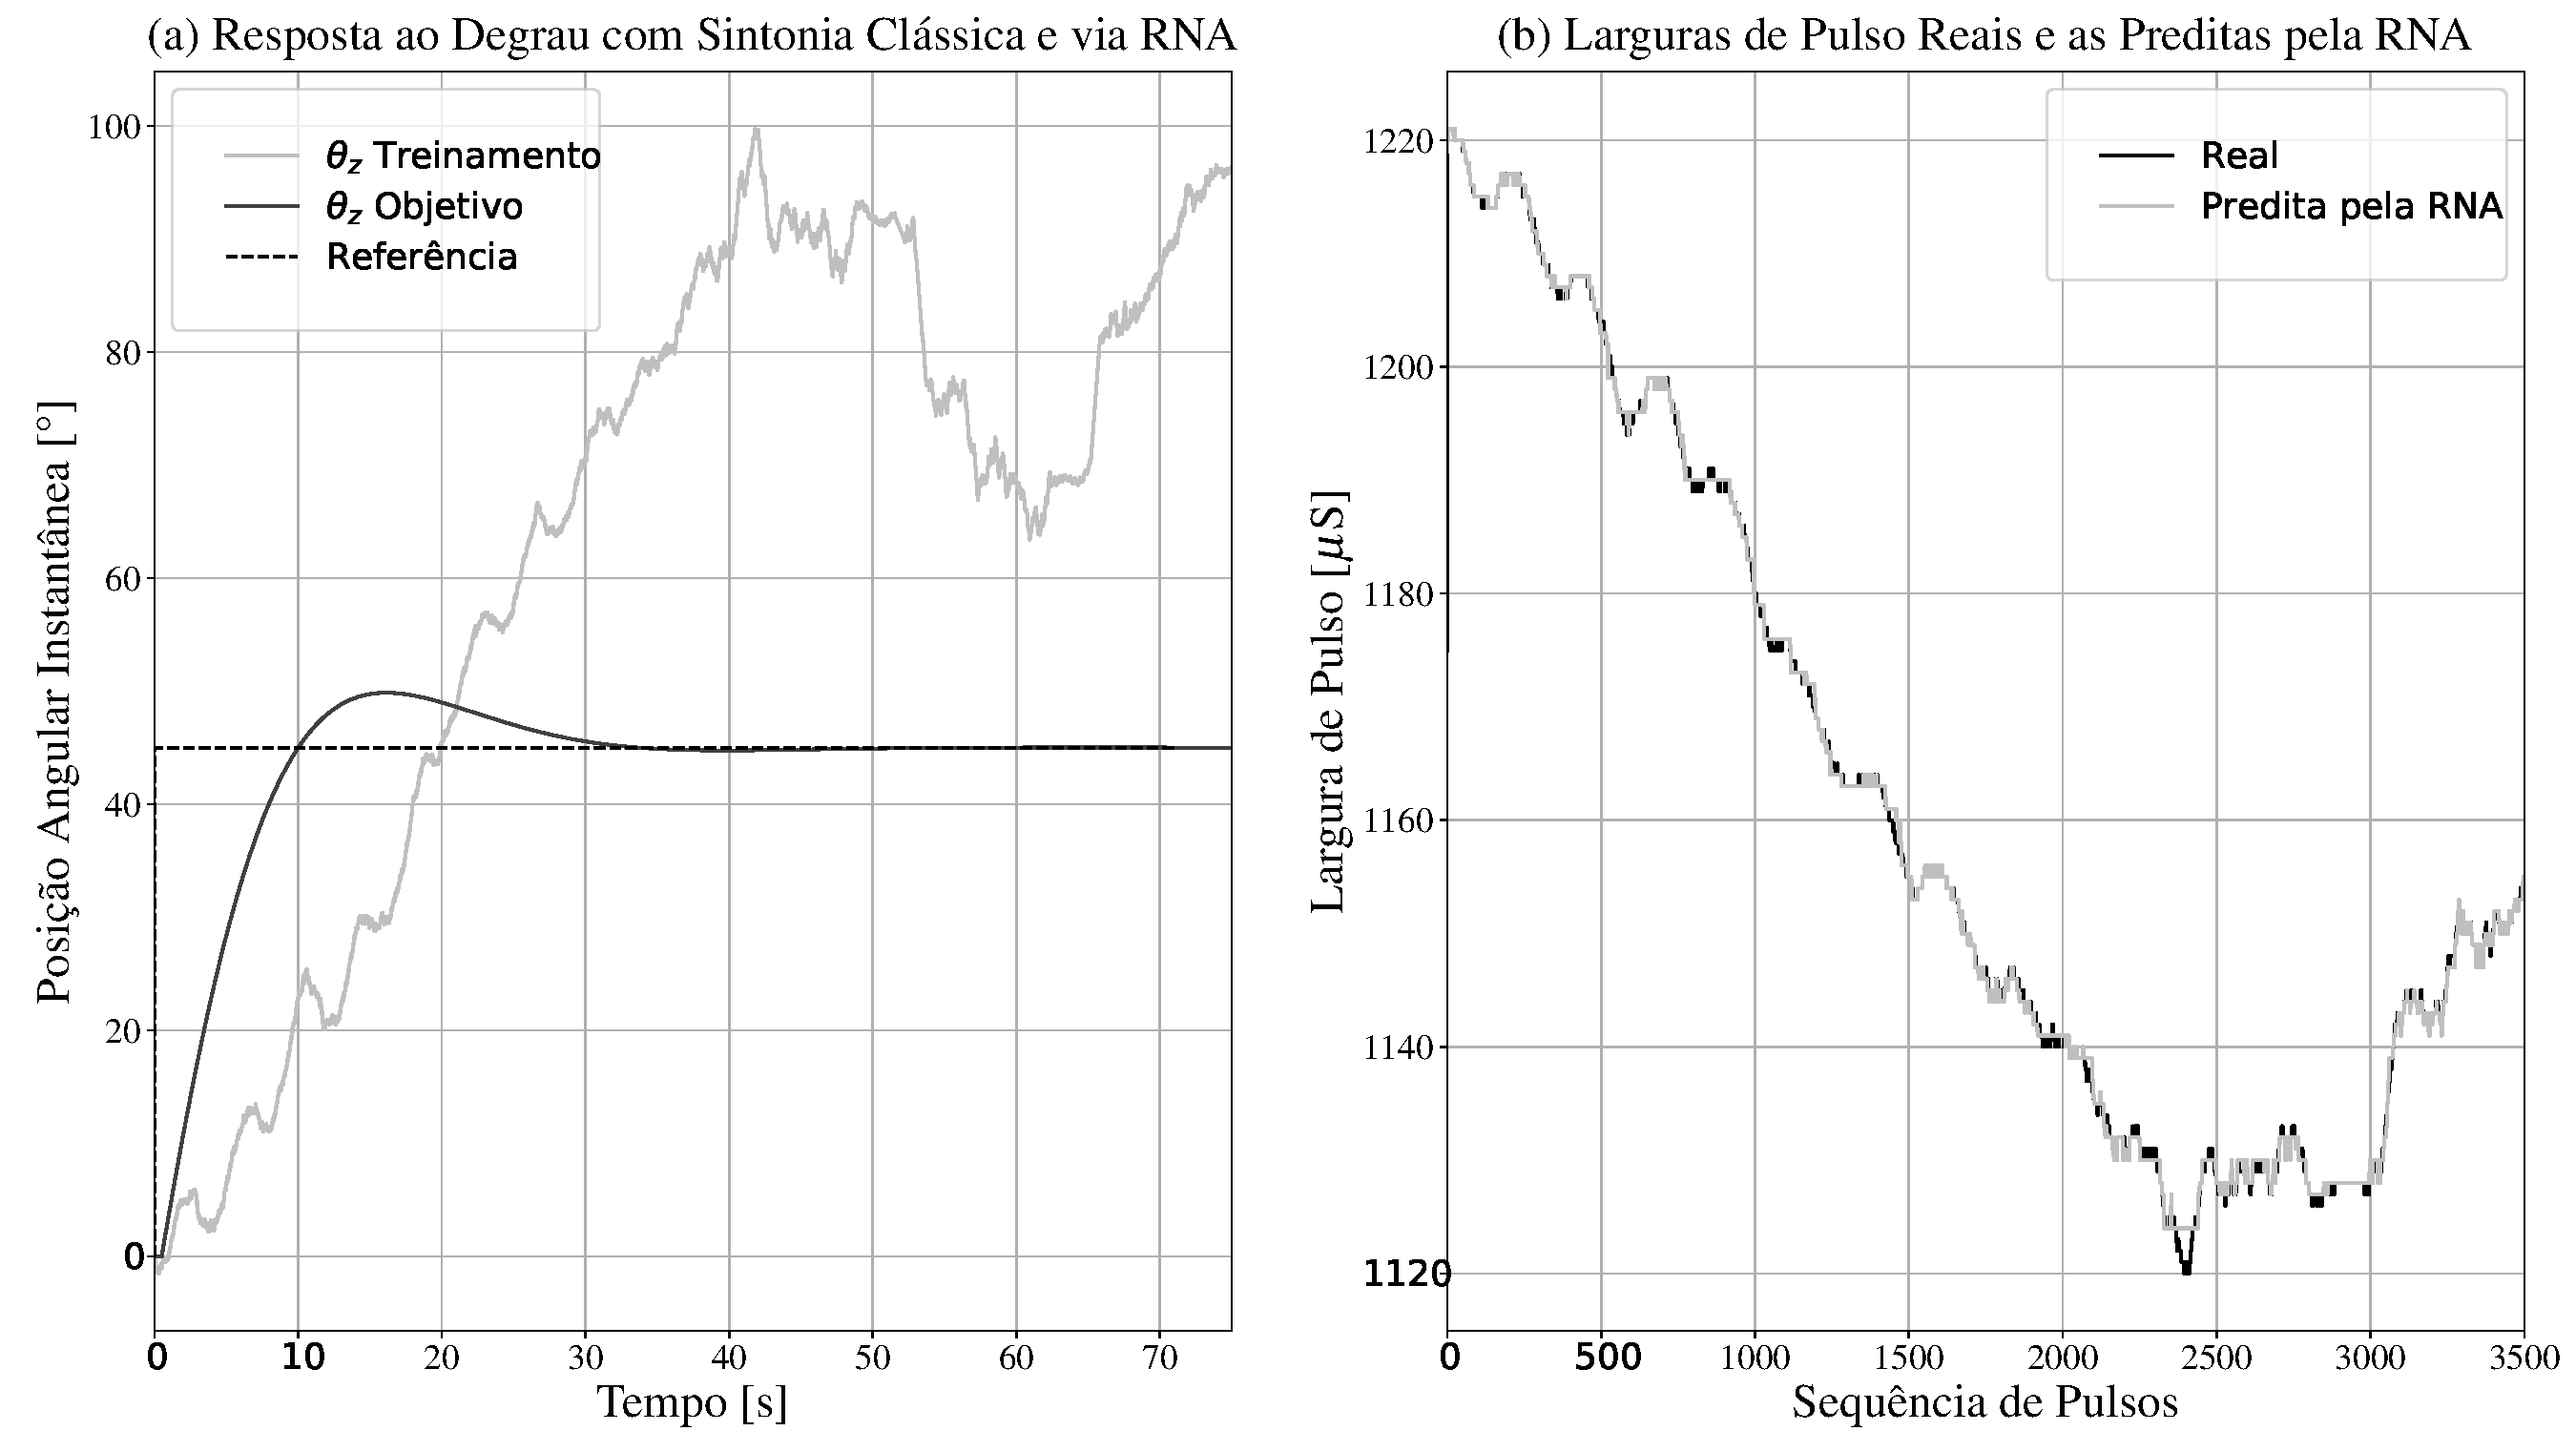
\includegraphics[scale=0.34]{resultados/img/neural_output}
  \end{center}
  \fonte{Elaborado pelo Autor.} 
  \label{fig:neural_output}
\end{figure}

Ainda, podemos observar na figura \ref{fig:neural_output} (a), onde podemos ver que o satélite oscila durante o regime transitório, como se acabasse retornando um pouco a cada novo avanço, isso é devido à rápida variação do sinal de controle que faz com que os motores perturbem o corpo com um torque contrário ao movimento, pois, a inércia do satélite é baixa e o atrito é desprezível devido ao mancal a ar. Já na figura \ref{fig:neural_output} (b), podemos ver o sinal do controlador predito pela RNA, juntamente com o sinal real amostrado no simulador de satélites. Com esses últimos dados, é possível se calcular o RMSE (\textit{Root Mean Square Error} - Erro quadrático médio) da seguinte forma:

\begin{equation}
RMSE = \sqrt{\frac{\sum_{t=1}^{T}(\hat{y}_t-y_t)^2}{T}}
\end{equation}

Onde T o número de amostras, $\hat{y}_t$ são os valores preditos pela RNA e $y_t$ são os valores reais. Assim obtemos o seguinte RMSE para a rede treinada:

\begin{equation}
RMSE \approx 1.0112
\end{equation}

O que é muito satisfatório, indicando que a RNA conta com um bom número de neurônio, número de camadas e interações. Após esses passo, podemos comparar todos os resultados, para uma análise mais objetiva. 


%%%%%%%%%%%%%%%%%%%%%%%%%%%%%%%%%%%

\subsection{Respostas ao degrau}

Após todos os métodos de sintonia aplicados, com foco no método do relé e no desenvolvido nesse trabalho, podemos comparar as respostas ao degrau. A figura \ref{fig:pid_result} (a) representa os resultados das simulações feitas na ferramenta Simulink, onde podemos ver os resultados da sintonia do controlador PID simples e com Anti-Windup.

\begin{figure}[H]
  \caption{Respostas ao degrau com sintonia via método do relé.}
  \begin{center}
      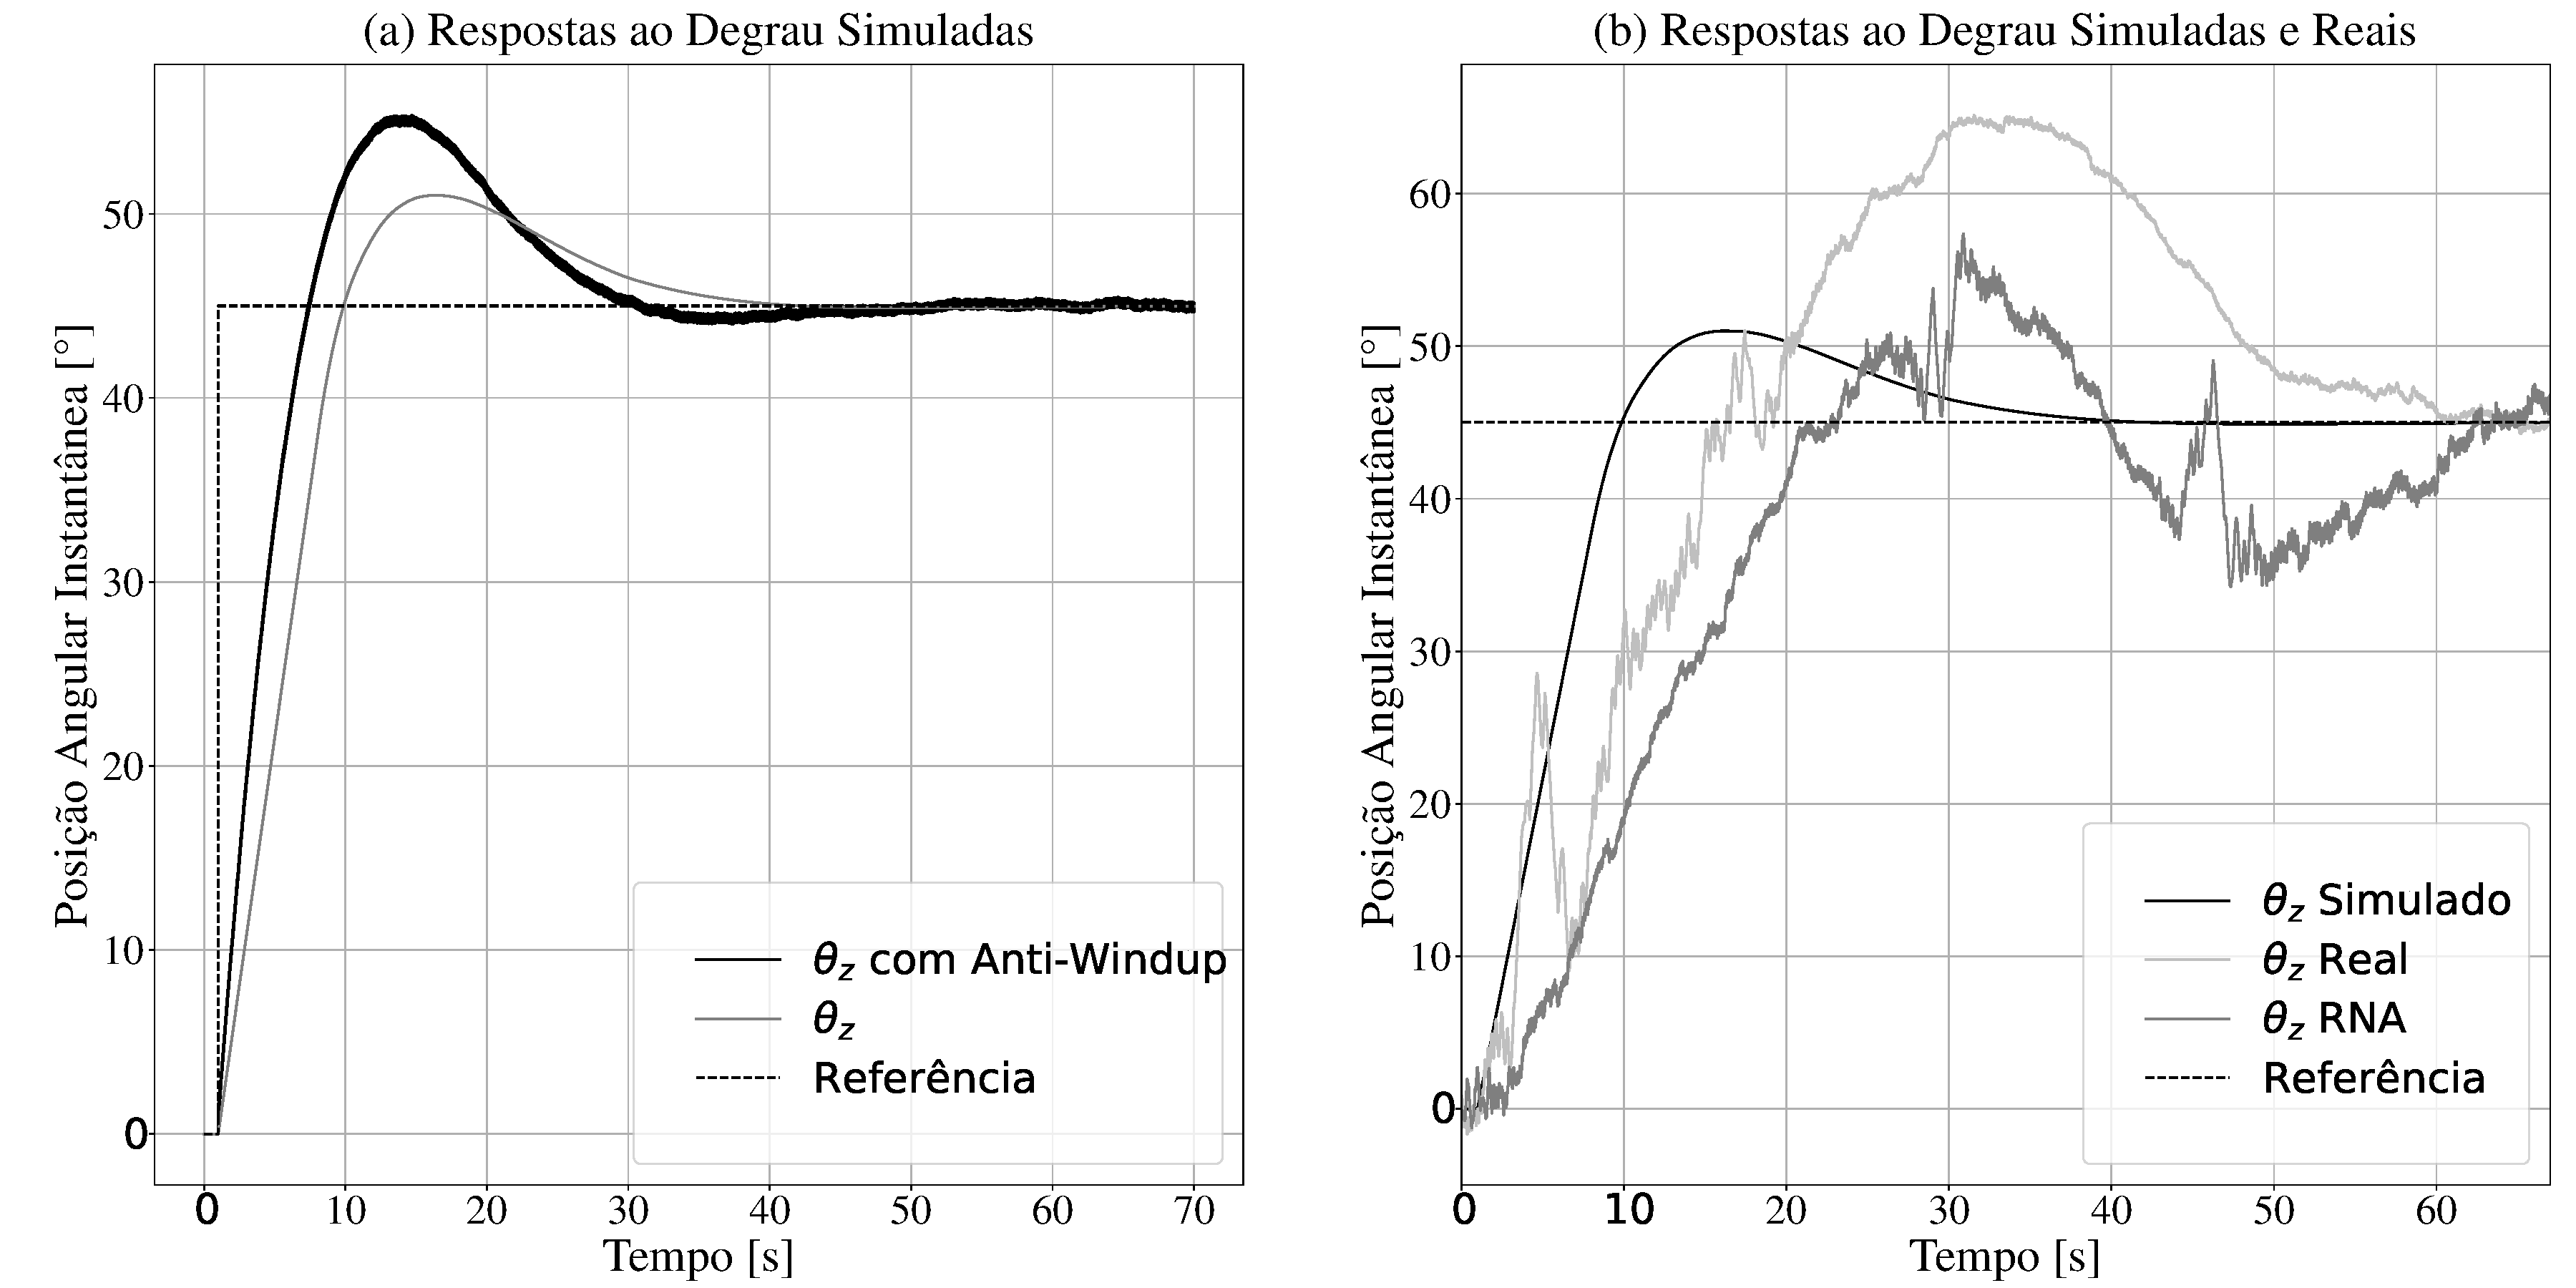
\includegraphics[scale=0.25]{resultados/img/pid_result}
  \end{center}
  \fonte{Elaborado pelo Autor.} 
  \label{fig:pid_result}
\end{figure}

Já na figura \ref{fig:pid_result} (b), podemos ver uma comparação entre o melhor resultado das simulações, ou seja, o controlador PID com Anti-Windup juntamente com o sinal real, também com Anti-Windup e sintonizado via RNA e regressão não-linear.

Como podemos ver, o sinal proveniente da simulação é mais rápido e com menor sobressinal. O sinal real com Anti-Windup apresentou o pior desempenho entre os três, pois teve o maior tempo de estabilização e sobressinal. O comportamento mais lento, maior sobressinal e mais ruidoso, se justifica pela presença de forças e perturbações que o modelo teórico não leva em consideração. Alguns problemas práticos que fazem o comportamento se desviar em relação ao teórico, são: a não perfeita simetria do simulador de satélites; perturbações pelo fluxo de ar no mancal, vibração excessiva dos motores, o que dificulta a aquisição de dados. Essa última pode ser vista na figura \ref{fig:pid_result_controlller} (a), onde podemos ver a velocidade angular em z da resposta real ao degrau, com um controlador PID com Anti-Windup. Percebe-se a grande presença de ruídos, muito mais do que pode ser visto na figura \ref{fig:bias_correction} (a), onde o simulador está estático.

\begin{figure}[H]
  \caption{Velocidade angular instantânea e sinal de controle.}
  \begin{center}
      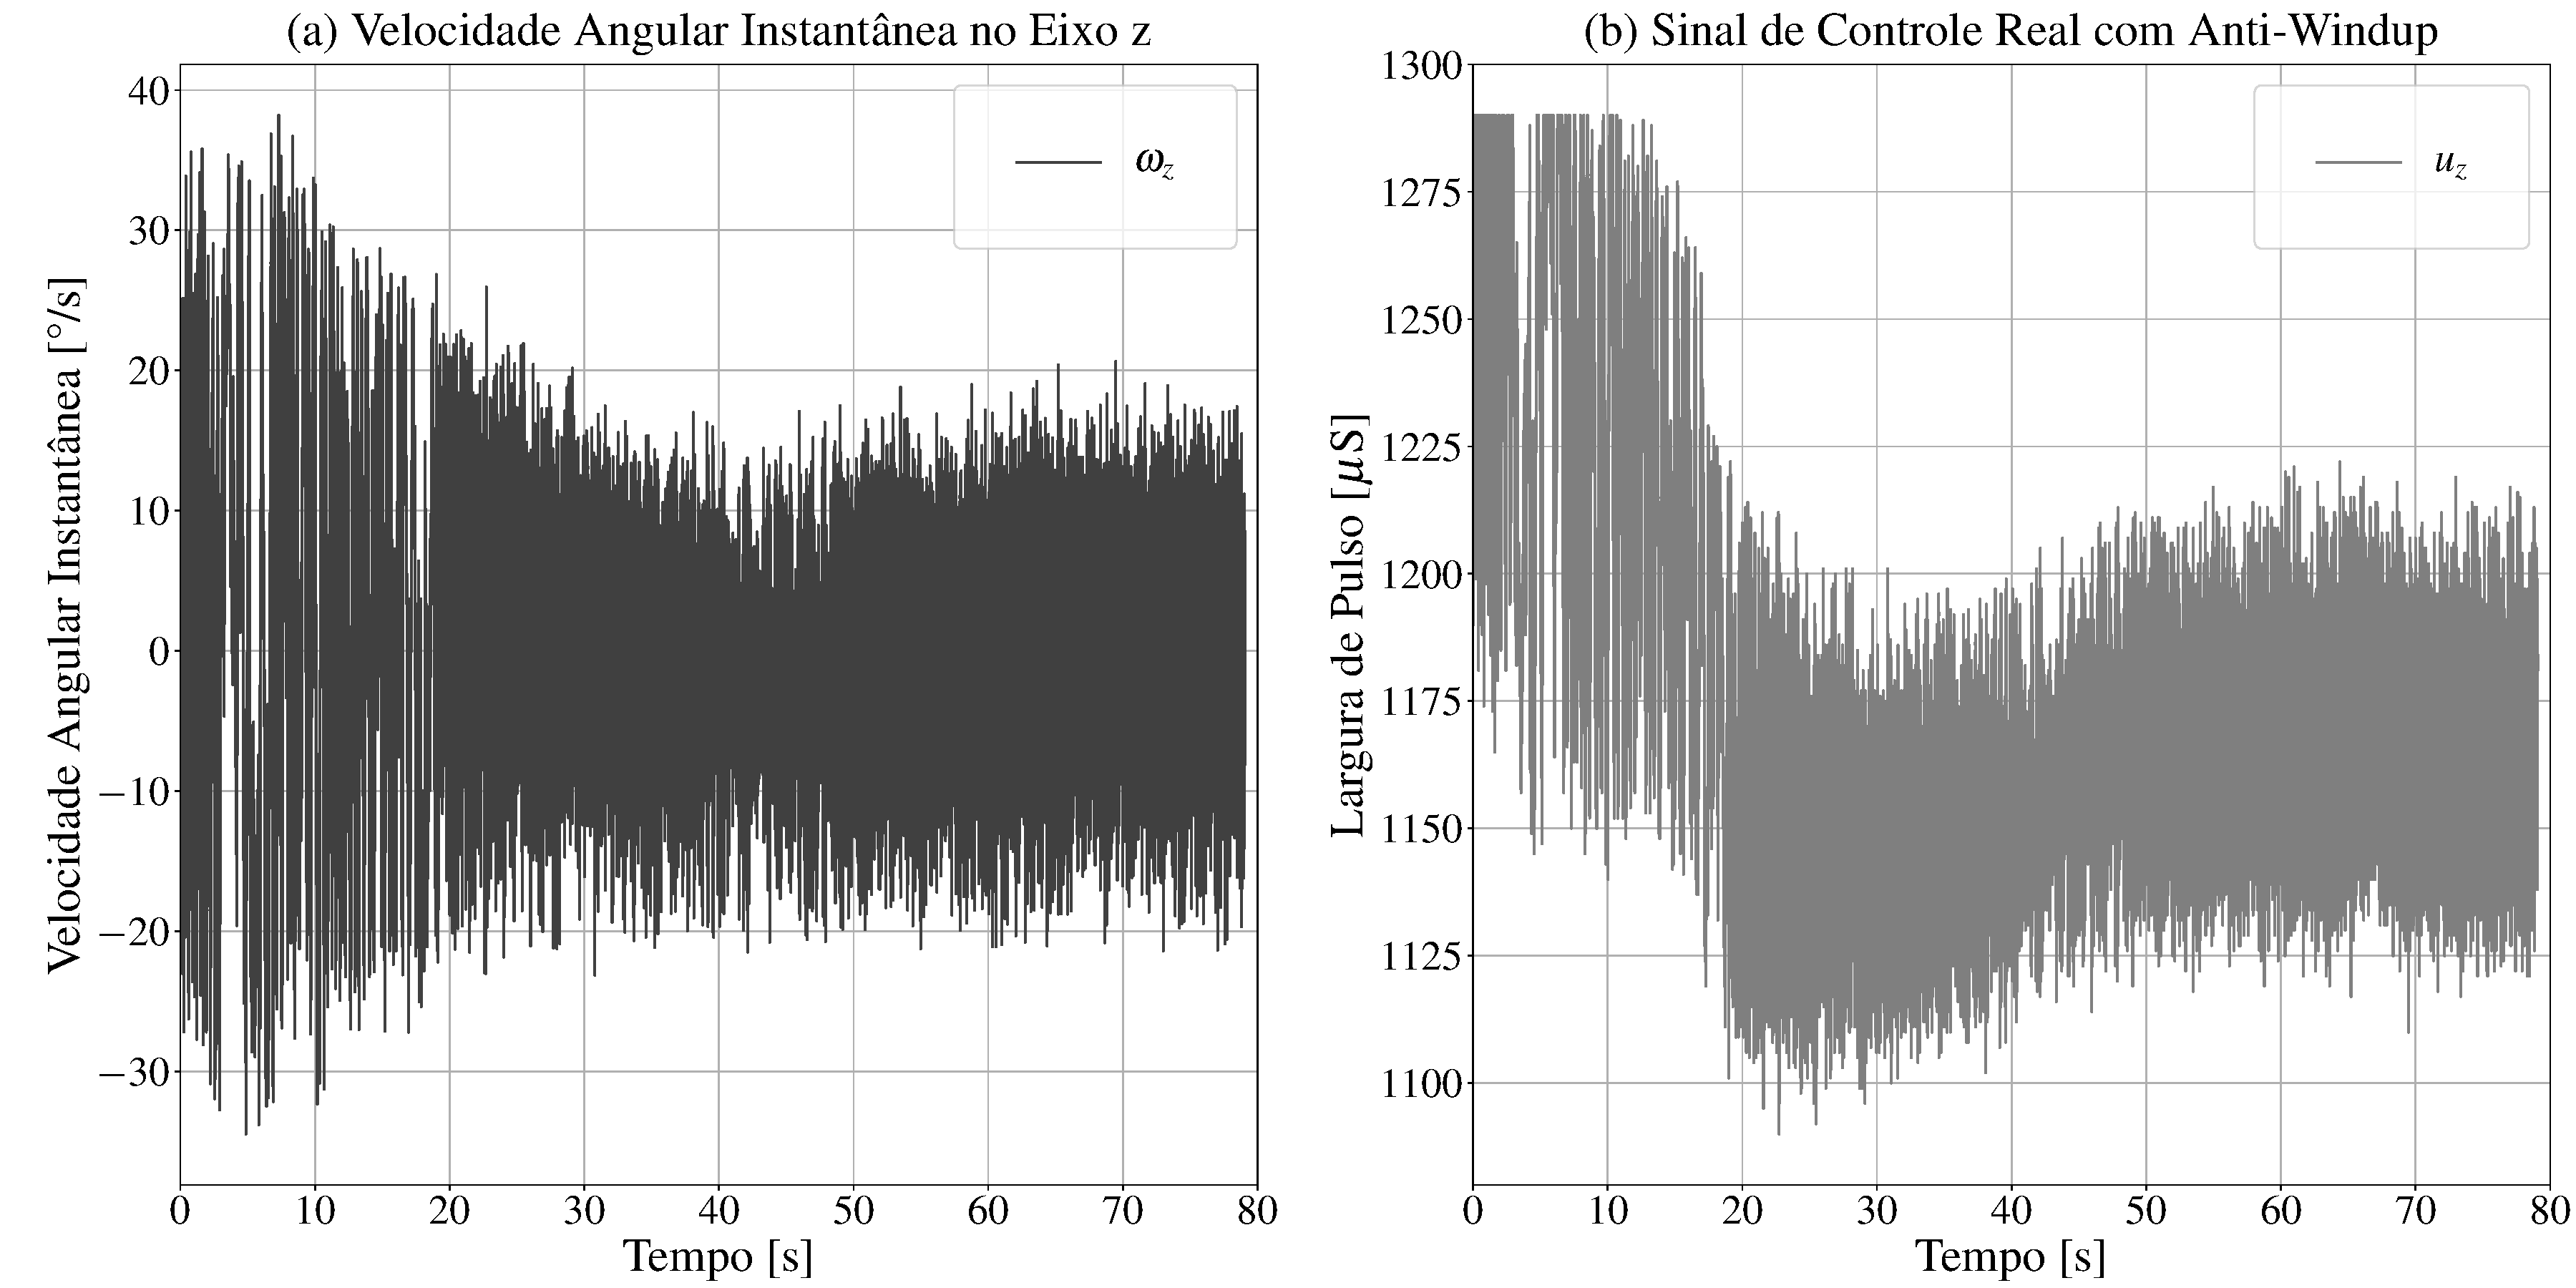
\includegraphics[scale=0.26]{resultados/img/pid_result_controller}
  \end{center}
  \fonte{Elaborado pelo Autor.} 
  \label{fig:pid_result_controlller}
\end{figure}

Por consequência, o sinal do controlador também apresentará grande quantidade de ruído, o que pode ser visto na figura \ref{fig:pid_result_controlller} (b), o que dificulta muito o controle. Sem a presença do filtro de Kalman devidamente ajustado, o controle não funcionaria de maneira adequada.

Desde o desenvolvimento mecânico, que exigiu a fabricação de todas as peças e além disso, ajustes para o perfeito funcionamento da dinâmica do simulador de satélites, os resultados foram funcionais e satisfatórios. O sistema de controle conseguiu manter uma performance que não influenciou nos resultados, mesmo que executado em um sistema operacional, que possuí escalonamento de tarefas, o que pode tornar a execução das tarefas não periódicas em muitos casos. E por fim, os resultados do método de sintonia desenvolvido usando RNA e regressão não linear, que otimizou de forma também satisfatória a resposta em relação aos métodos clássicos de sintonia.
